% !TeX root = ../main.tex

\chapter{基于3D高斯泼溅的水下三维重建}
3D 高斯泼溅(3DGS)\cite{3DGS} 已逐步取代神经辐射场(NeRF)\cite{nerf} 技术,成为场景重建领域的热门工具。
然而,目前尚缺乏针对水下环境的充分验证与应用研究,主要原因在于缺少专门用于此类任务的水下场景数据集支持。
此外,由于水下图像的退化效应(如光散射、色偏)及水流造成的动态扰动,水下场景重建需要超越静态场景重建的传统方法。
得益于神经网络的时空预测能力,3DGS 在动态场景的重建中也具备高质量的场景复现能力。
为此,本章提出了一种基于 3DGS 和 KAN \cite{kan}变形扩展的水下场景感知增强框架。
该框架旨在优化特定时刻下的静态场景表示,通过抑制运动干扰从而保留水下场景的基础静态特征。
同时,本章构建了一个专门面向水下场景重建的数据集,并在此数据集上对方法进行验证。
实验结果表明,与其他基准方法相比,本章提出的框架在准确性和鲁棒性方面具有显著优势。

\section{水下动态场景的3D高斯泼溅方法} \label{sec:4dgs}
3D 高斯泼溅方法可以直接对场景信息进行显式表示,这为动态场景建模提供了一种灵活的解决方案。
其核心思想是通过变形每个时间点的 3D 高斯表示,寻找符合动态场景重建的最优变形方法。
目前,利用神经网络学习位置与时间信息的映射关系已成为主流方案。
在此基础上,本章基于时空信息编码与解码的4D高斯泼溅\cite{4DGS}框架为水下动态场景重建提供有效支持。
如图\ref{img:4dgs}所示,该框架通过时空结构编码器高效提取 3D 高斯的时空特征,并结合特征解码器实现高斯变形预测,从而提升水下动态场景重建的质量和效率。
\begin{figure}[htbp]
    \centering
    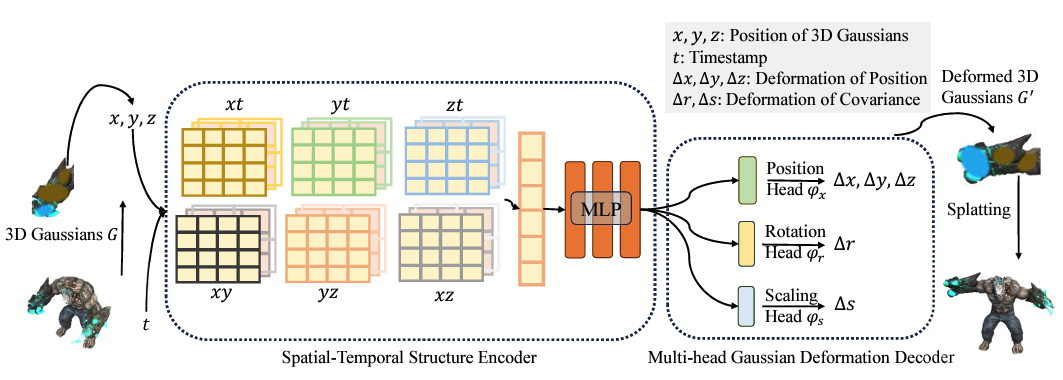
\includegraphics[width=0.8\textwidth]{figures/ch4/4dgs.jpg}
    \caption{基于 3D 高斯泼溅的水下动态场景重建框架}
    \label{img:4dgs}
\end{figure}

\subsection{3D高斯时空编码器}
动态场景中的相邻 3D 高斯通常具有显著的时空信息相似性。
为高效捕捉这些相似性特征,本章设计了一种时空结构编码器 $\mathcal{H}$,
该编码器由多个分辨率的 HexPlane 模块\cite{hex_plane} 和一个多层感知机(MLP)模块组成。
其主要目标是结合 3D 高斯的位置与时间信息,将其映射到低维特征空间,为后续多头解码器进行变形预测提供支持。

为了避免高维空间的维度灾难,本章的HexPlane模块采用了K-Planes\cite{k-planes}的方法将每个点的特征分解为它在空间中的特征和它在每个轴(XYZ)上关于时间的特征,从而优化内存占用并降低计算复杂度。
具体做法是将原始 4D 神经体素分解为 6 个独立的平面模块,这些模块能够有效表示一定区域内的 3D 高斯,并通过时间维度进一步捕捉高斯变形信息。
因此3D时空结构编码器$\mathcal{H}$包含6个多分辨率平面模块$R_l(i,j)$和一个小型MLP模块$\phi_d$,如公式\ref{eq:encoder_H}所示:
\begin{equation}
\label{eq:encoder_H}
\mathcal{H}(\mathcal{G}, t) = \{ R_l(i,j), \phi_d \ | \ (i,j) \in \{(x,y), (x,z), (y,z), (x,t), (y,t), (z,t)\}, l \in \{1, 2\} \}
\end{equation}

其中,$\mathcal{X} = (x, y, z)$表示3D高斯的中心位置,$l$表示上采样的尺度,
$R(i,j)$是每个体素平面模块,维度为$R(i,j) \in \mathbb{R}^{h \times l N_i \times l N_j}$,
其中$h$表示平面中单个网格特征的维度,$N_i,N_j$表示每个平面体素网格的基本分辨率。

为提取每个体素特征,需要在6个2D体素平面中对3D高斯体的信息进行编码,可以使用双线性插值的方法查询平面体素网格四个顶点的特征,计算公式为:
\begin{equation}
f_h = \bigcup_l \prod \text{interp}(R_l(i,j)), \quad (i,j) \in \{(x,y),(x,z),(y,z),(x,t),(y,t),(z,t)\}
\end{equation}

其中,$f_h \in \mathbb{R}^{h \times l}$表示神经体素的特征。
随后,MLP 模块 $\phi_d$ 融合所有特征以生成最终的编码表示:
\begin{equation}
f_d = \phi_d(f_h)
\end{equation}  

该编码过程不仅可以高效捕获动态场景中时空特征的变化,还为后续高斯变形计算奠定基础。

\subsection{基于KAN的特征解码器}
时空结构编码器生成的 3D 高斯特征随后被输入到多头高斯变形解码器 $\mathcal{D}$ 中,以计算每个 3D 高斯在不同时刻下的变形信息。
该解码器包含多个KAN模块,分别用于估计位置变形$\Delta \mathcal{X}$、旋转变形$\Delta r$和缩放变形$\Delta s$。
这些变形信息构成了变形后的 3D 高斯表示$\mathcal{G}^\prime=\{\mathcal{X}^\prime, s^\prime, r^\prime, \sigma, \mathcal{C} \}$。
KAN 模块通过学习神经元的最优激活方式,在保证解码准确性的同时减少了所需的神经元数量。
基于KAN的特征解码器通过自适应的方式预测形变量,最终的变形3D高斯可以表示为:
\begin{equation}
    \mathcal{G}^\prime = \{ \mathcal{X} + \Delta \mathcal{X}, r + \Delta r, s + \Delta s, \alpha + \Delta \alpha, \mathcal{C} + \Delta \mathcal{C} \}
\end{equation}

不同时刻下的3D高斯可以有效处理水下环境中的动态特征,生成精准的动态场景重建结果。

\section{水下静态三维场景自对抗训练}
\subsection{多阶段训练模式}
在水下复杂环境中,水流引发的动态干扰会导致场景中物体晃动,使得完全静态的水下场景重建变得极具挑战性。
尽管基于动态场景重建的方法能够在一定程度上保留动态效果并生成高质量、逼真的新视图,
但在单目相机拍摄的水下动态场景中,某些时刻可能出现异常的重建现象。这种现象通常由以下原因导致:
(1)某些时刻运动干扰过于强烈,画面质量显著下降;
(2)动态场景数据集中缺乏足够的视角覆盖,导致 3D 高斯变形预测出现误差。

真实世界中水下重建场景的对象位置相对固定,且水流带来的扰动具有一定周期性,导致不同视角下的场景存在相似的高频信息。
为捕捉这些高频静态特征并实现高质量水下场景重建,本章提出了一种带有场景过滤模块的多阶段训练模式。
如图 \ref{img:3_stage}和算法\ref{alg:3_stage} 所示,该模式分为以下三个阶段:初始化训练阶段、动态场景训练阶段和目标场景训练阶段。
\begin{figure}[htbp]
    \centering
    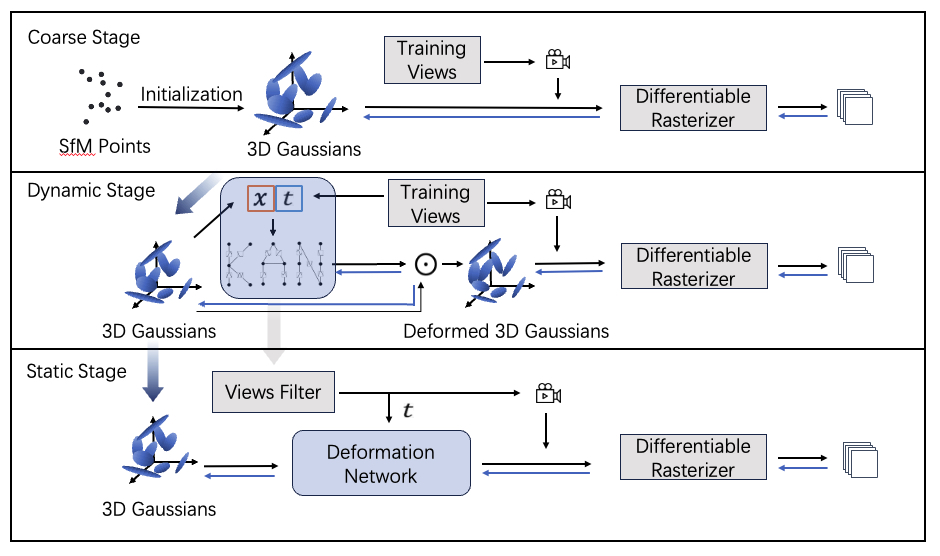
\includegraphics[width=0.8\textwidth]{figures/ch4/3_stage.jpg}
    \caption{多阶段训练模式}
    \label{img:3_stage}
\end{figure}

\begin{algorithm}[t]
    \caption{\label{alg:3_stage}训练流程}
    \KwIn{$Cams$: 原始训练摄像机}
    
    \tcp{初始化训练阶段}
    $\mathcal{G} = Train_{w/o\_\mathcal{F} }(Cams)$\;

    \tcp{动态场景训练阶段}
    $\mathcal{G}, \mathcal{F} = Train_{w/\_\mathcal{F} }(Cams)$\;

    \tcp{场景过滤}
    $StaticCams = Filter(\mathcal{G}, Cams, d, \mathcal{F})$\;

    \tcp{目标场景训练阶段}
    $\mathcal{G}, \mathcal{F} = Train_{w/\_\mathcal{F} }(StaticCams)$\;
\end{algorithm}

(1)初始化训练阶段:利用基于结构化运动(SfM)方法\cite{sfm1}\cite{sfm2}初始化的点云,对 3D 高斯初始表示进行训练。该阶段旨在快速完成初步重建,缓解动态重建初期的不稳定性。
(2)动态场景训练阶段:通过章节 \ref{sec:4dgs} 中介绍的 3D 高斯时空编码器与基于 KAN 的特征解码器对动态场景进行训练,从而提高水下动态重建质量,同时保留动态效果。
(3)目标场景训练阶段:通过场景过滤模块筛选动态场景训练结果,剔除低重复度的异常数据,提取相对固定的高频信息。最终实现目标静态场景的高质量重建。
这种多阶段模式的设计,不仅有效分离了动态和静态信息,还显著提升了静态场景的重建精度和稳定性。

\subsection{场景过滤模块}
如算法 \ref{alg:filter} 所示,为确保在目标水下静态场景训练阶段能够高效筛选出静态特征,同时避免过度占用内存资源,
本章设计了空间点云双重遍历机制来优化数据选择:
(1)第一次遍历:对所有时刻的 3D 高斯数据进行累加求和,计算每个 3D 高斯的平均位置,并将其作为过滤的基准。
(2)第二次遍历:筛选出与平均位置相似的数据,并记录这些时刻 $t_{static}$,以保留高斯高度相似的静态对象。
\begin{algorithm}[t]
    \caption{\label{alg:filter}场景过滤模块(Filter)}
    \KwIn{$\mathcal{G}$: 三维高斯分布,$cams$: 原始训练摄像机,$d$: 距离阈值,$\mathcal{F}$: 形变模型}
    
    $\mathcal{X} = \text{GetPoints}(\mathcal{G})$\tcp*{获取三维高斯分布的点集}
    $s = \text{GetScale}(\mathcal{G})$\tcp*{获取缩放参数}
    $r = \text{GetRotation}(\mathcal{G})$\tcp*{获取旋转参数}
    $\alpha = \text{GetOpacity}(\mathcal{G})$\tcp*{获取不透明度}
    $\mathcal{C} = \text{GetSphericalHarmonics}(\mathcal{G})$\tcp*{获取球谐系数}
    
    \tcp{计算场景的静态位置}
    \For{每个 $cam$ $\in$ $cams$}{
        $\mathcal{X}_{\text{cam}} = \mathcal{F}(\mathcal{X}, s, r, \alpha, \mathcal{C}, cam)$\tcp*{计算当前摄像机的点集}
        $\mathcal{X}_{\text{cum}} = \mathcal{X}_{\text{cum}} + \mathcal{X}_{\text{cam}}$\tcp*{累积点集}
    }
    $\mathcal{X}_{\text{center}} = \mathcal{X}_{\text{cum}} / \text{len}(cams)$\tcp*{计算场景的中心位置}
    
    \tcp{筛选距离小于 $d$ 的静态摄像机}
    \For{每个 $cam$ $\in$ $cams$}{
        重新计算 $\mathcal{X}_{\text{cam}}$ 而不是存储其值\tcp*{重新计算点集}
        $\mathcal{X}_{\text{cam}} = \mathcal{F}(\mathcal{X}, s, r, \alpha, \mathcal{C}, cam)$\tcp*{计算当前摄像机的点集}
        $d_{\text{cam}} = \text{ComputeDistance}(\mathcal{X}_{\text{cam}}, \mathcal{X}_{\text{center}})$\tcp*{计算到中心位置的距离}
        \If{$d_{\text{cam}} < d$}{
            \tcp{将当前摄像机添加到静态摄像机集合中}
            $StaticCams = \text{AddStaticCameras}(cam)$
        }
    }
    \Return $StaticCams$\tcp*{返回静态摄像机集合}
\end{algorithm}

如图 \ref{img:filter} 所示,该过滤模块能够从不同时刻的 3D 高斯数据中有效提取高频静态信息,为目标静态场景训练提供可靠的数据支持。
此外,为降低因过滤误差引发的潜在影响,本章在静态训练阶段保留了动态重建的变形机制,引入时序信息增强了对异常数据的宽容度。
这种设计在水下复杂环境中,显著提高了静态场景重建的鲁棒性和可靠性。
\begin{figure}
    \centering
    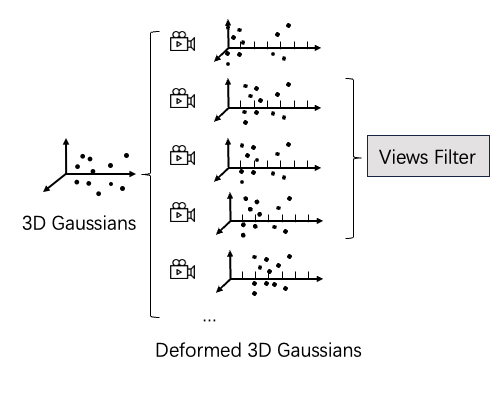
\includegraphics[width=0.8\textwidth]{figures/ch4/filter.jpg}
    \caption{场景过滤模块}
    \label{img:filter}
\end{figure}

\subsection{损失函数设计}
与其他重建方法类似\cite{3DGS}\cite{tineuvox}\cite{dnerf},本文采用L1颜色损失(L1 Color Loss)来监督训练过程,
确保生成的3D高斯在颜色方面与目标场景的实际颜色保持一致。
此外,还引入了基于网格的全变差损失(Total Variation Loss,$\mathcal{L}_{tv}$),
以减少噪声并提高重建结果的平滑性。

L1颜色损失用于衡量生成的场景颜色与真实场景颜色之间的绝对误差,计算公式为:
\begin{equation}
    \mathcal{L}_{color} = \sum_{i} \left\| \hat{C}_i - C_i \right\|_1
\end{equation}

其中,$\hat{C}_i$是模型生成的第$i$个像素的颜色值,$C_i$是对应的真实颜色值。

全变差损失通过度量网格中像素值的梯度变化来减少不必要的细节和噪声,从而增强重建结果的平滑性和稳定性,特别是在处理高频细节和复杂动态场景时。
其计算公式为:
\begin{equation}
    \mathcal{L}_{tv} = \sum_{i,j} \left\| \nabla \mathcal{G}(i,j) \right\|_2
\end{equation}

其中,$\nabla \mathcal{G}(i,j)$表示网格中位置$(i,j)$的梯度,衡量的是相邻体素之间的变化。这个损失项在训练过程中有助于避免模型过度拟合细节,从而提高重建的鲁棒性。

最终的总损失函数 $\mathcal{L}_{total}$ 结合了上述两种损失,通过加权组合实现颜色一致性与平滑性的平衡:
$$
\mathcal{L}_{total} = \mathcal{L}_{color} + \lambda_{tv} \cdot \mathcal{L}_{tv}
$$

其中,$\lambda_{tv}$是全变差损失的权重系数,用于平衡颜色损失和平滑性损失之间的影响。
通过最小化总损失函数,模型不仅能够实现对动态场景的高精度重建,还能有效抑制噪声的干扰,保证生成结果的平滑性和视觉质量。

\section{实验结果}
\subsection{水下重建数据集制作}
为验证水下重建方法的有效性,本章制作了一个专用水下重建数据集 3DUW。
首先,搭建了一个可控的人造水下场景,并通过组合不同的环境条件(水流扰动和色偏)生成四组配对数据集,以测试算法在动态扰动抑制和颜色校正(去色偏)能力上的表现。
如图 \ref{img:3DUW} 所示,不同环境条件下的数据集为算法的泛化性能验证提供了丰富的场景样本。
随后,使用单目相机从多个角度和时间点采集水下场景图像,应用SfM算法\cite{sfm1}\cite{sfm2}对数据进行预处理,生成每张图像对应的相机位姿信息和初始点云。
\begin{figure}
    \centering
    \includegraphics[width=0.8\textwidth]{figures/ustc-badge.pdf}
    \caption{3DUW 数据集}
    \label{img:3DUW}
\end{figure}

另外,由于3DGS的重建质量在很大程度上依赖于SfM中获得的初始点云。
而水下原始图像由于存在不同程度的模糊和色偏,导致SfM算法难以提取准确的特征点,只会产生稀疏的点云。
为了形成一个更加密集的点云,在获取水下图像后,使用K-Nearest-Neighbor(KNN)算法在现有点的外围添加额外的点。
算法\ref{eq:knn}描述了向原有稀疏点云添加补充点的过程。
\begin{algorithm}[t]
    \caption{\label{eq:knn}添加额外点云}
    \KwIn{$\mathcal{G}$: 从 SfM 计算的点云}
    \KwIn{$K$: 需要查找的邻近点个数}
    \KwIn{$N_p$: 需要生成的额外点个数}
    \KwIn{$t_d$: 新生成点与已有点之间的最小距离要求}
    
    $P_\text{add} \leftarrow \text{GenerateRandomPoints}(\mathcal{P}, N_p)$\tcp*{均匀采样生成 $N_p$ 个新点}
    
    \For{每个 $p \in P_\text{add}$}{
        $\mathcal{P}_\text{knn} \leftarrow \text{FindNearestNeighbors}(\mathcal{P}, p, K)$\tcp*{找到 $p$ 在 $\mathcal{P}$ 中的 $K$ 个最近邻点}
        $\mathcal{P}_\text{valid} \leftarrow \text{CheckDistance}(\mathcal{P}_\text{knn}, p, t_d)$\tcp*{筛选出与 $p$ 距离满足要求的邻居点}
    
        \If{$|\mathcal{P}_\text{valid}| > 0$}{
            $p_c \leftarrow \text{LinearInterpolate}(\mathcal{P}_\text{valid}, p)$\tcp*{线性插值生成新点的颜色}
            $\text{AddToPointCloud}(\mathcal{P}, p, p_c)$\tcp*{将新点添加到点云 $\mathcal{P}$ 中}
        }
    }
\end{algorithm}

首先,通过均匀采样的方法在点云范围内生成$N_p$个随机的新点$P_\text{add}$。对于每个新点$p$,算法利用KNN方法从初始点云中找到其K个最近邻点,构成候选邻域集合$\mathcal{P}\text{knn}$。
随后,通过检查邻近点与新点之间的距离,通过$t_d$筛选出满足最小距离要求的有效邻居点集合$\mathcal{P}\text{valid}$。
如果有效邻居点集合非空,算法通过对有效邻居点的颜色信息进行线性插值,估算新点的颜色属性,并将该点及其颜色属性添加到点云中,完成补充点的生成。
这样的操作确保了新增点既满足稠密性需求,又与原始点云保持一致的几何和颜色特性。
该算法通过逐点更新的方式动态扩展了点云密度,同时有效避免了新增点与原始点过度重叠或无效分布的问题,为水下重建提供了更加丰富且高质量的点云数据支撑。

\subsection{实验设置}
为验证本章提出水下三维重建方法的性能和鲁棒性,实验选用了两组真实水下数据集:自制的 3DUW 数据集和公开数据集 SeaThru-NeRF\cite{seathru}。两组数据集的划分如表 \ref{tab:recondata_split} 所示。
\begin{table}[htbp]
    \centering
    \caption{水下重建数据集划分}
    \label{tab:recondata_split}
    \begin{tabular}{cccc}
        \toprule
        数据集 & 训练集 & 验证集 & 共计 \\
        \midrule
        3DUW-1 & 200 & 50 & 50 \\
        3DUW-2 & 200 & 50 & 50 \\
        3DUW-3 & 200 & 50 & 50 \\
        3DUW-4 & 200 & 50 & 50 \\
        SeaThru-NeRF-1 & 100 & 25 & 25 \\
        SeaThru-NeRF-2 & 100 & 25 & 25 \\
        SeaThru-NeRF-3 & 100 & 25 & 25 \\
        \bottomrule
    \end{tabular}
\end{table}
实验的时空编码器与解码器均基于 PyTorch 框架\cite{pytorch}实现,利用其高效的深度学习工具链保证了模型的开发与训练效率。
所有实验均在单张 RTX 3060 GPU 上完成,初始化训练、动态场景训练和目标场景训练的迭代次数分别设置为 3000 次、20000 次和 10000 次。

\subsection{定量评价}
为全面评估水下场景重建方法的性能,实验采用除章节\ref{sec:quantitative}中的参考指标PSNR与SSIM外,还包含一下指标:
(1)感知质量指标(LPIPS)\cite{lpips}:LPIPS 使用预训练的深度网络来提取图像特征,然后计算这些特征之间的距离,以评估图像之间的感知相似度;
(2)运行帧率(FPS):衡量模型在重建渲染时的速度。

实验对包括 TiNeuVox\cite{tineuvox}、3DGS\cite{3DGS}、4DGS\cite{4DGS}和 Sea-NeRF\cite{seathru}
的多个先进方法进行了比较,实验结果见表 \ref{tab:res_3duw}和\ref{tab:res_seanerf},
需要指出的是,由于我们的方法引入了场景过滤模块,测试集上的实验仅比较场景过滤模块筛选后的数据,以确保评价的公平性和一致性。
\begin{table} [htbp]
    \small
    \centering
    \caption{Quantitative results on the 3DUW dataset. }
    \setlength{\tabcolsep}{10pt}
    \begin{tabular}{lcccccc} 
    \toprule
    Model  & PSNR(dB)↑ & SSIM↑ & LPIPS↓ & Time↓ &  FPS ↑  \\
    \midrule  
    TiNeuVox~\cite{tineuvox}  & 32.67 & 0.97 &  0.04 & 45 mins & 0.79\\ 
    3DGS~\cite{3DGS} &23.19 & 0.93 & 0.08&22 mins  &94\\
    4DGS\cite{4DGS} & 34.05&0.98 &0.02& 29 mins&42 \\
    Sea-NeRF\cite{seathru} & 34.58 & 0.98 & 0.02 & 38 mins & 45\\
    Ours & 34.58 & 0.98 & 0.02 & 38 mins & 45\\
    \bottomrule
    \end{tabular}  
    \label{tab:res_3duw}
\end{table}
    
\begin{table} [htbp]
    \small
    \centering
    \caption{Quantitative results on the SeaThru-NeRF dataset. }
    \setlength{\tabcolsep}{10pt}
    \begin{tabular}{lcccccc} 
    \toprule
    Model  & PSNR(dB)↑ & SSIM↑ & LPIPS↓ & Time↓ &  FPS ↑  \\ 
    \midrule  
    TiNeuVox~\cite{tineuvox}  & 32.67 & 0.97 &  0.04 & 45 mins & 0.79\\ 
    3DGS~\cite{3DGS} &23.19 & 0.93 & 0.08&22 mins  &94\\
    4DGS\cite{4DGS} & 34.05&0.98 &0.02& 29 mins&42 \\
    Sea-NeRF\cite{seathru} & 34.58 & 0.98 & 0.02 & 38 mins & 45\\
    Ours & 34.58 & 0.98 & 0.02 & 38 mins & 45\\
    \bottomrule
    \end{tabular}  
    
    \label{tab:res_seanerf}
\end{table}

\subsection{主观评价}
如图 \ref{img:res_3duw} 所示,在静态数据集 Sea-NeRF 上,本章方法的重建结果与其他方法的表现几乎一致。
然而,在具有动态干扰的 3DUW 数据集中,本文方法展现出了显著优势,
通过场景过滤模块能够有效筛选出因水流扰动导致的不利数据,这些数据点通常会对其他正常训练数据的视觉细节产生负面影响。
通过剔除这些不利数据,本文方法成功保留了目标场景的完整性,显著提升了动态场景重建的整体质量。
相比之下,其他具备动态重建能力的方法(如 TiNeuVox\cite{tineuvox}、4DGS\cite{4DGS})虽然在动态场景中能够生成高质量的新视角,
但在某些特定时刻和视角下,其渲染效果不够稳定。
实验证明场景过滤模块在这种情况下能够通过优化数据质量,确保生成的动态新视角在不同时间点和视角下都保持较高的一致性和细节还原度。
\begin{figure}[htbp]
    \centering
    \includegraphics[width=0.8\textwidth]{figures/ustc-badge.pdf}
    \caption{水下重建结果对比}
    \label{img:res_3duw}
\end{figure}

\subsection{结果讨论}
\subsubsection{消融实验}
(1)KAN:
如表\ref{tab:recon_ablation}所示,与传统的基于多层感知机的特征解码器相比,KAN对最终渲染结果的质量具有一定的提升。
(2)场景过滤模块:
场景过滤模块在动态场景训练阶段结束后执行数据筛选,剔除干扰性数据。
如表\ref{tab:recon_ablation}所示,场景过滤模块有效消除了由水流运动引起的视觉细节误差,渲染细节并增强整体渲染质量。
\begin{table}
    \centering
    \caption{消融实验结果}
    \label{tab:recon_ablation}
    \begin{tabular}{lcc}
        \toprule
        模型 & PSNR(dB)↑ & SSIM↑ \\
        \midrule
        3DGS & 23.19 & 0.93 \\
        3DGS + KAN & 24.05 & 0.94 \\
        3DGS + KAN + Filter & 34.58 & 0.98 \\
        \bottomrule
    \end{tabular}
\end{table}


\subsubsection{局限性}
尽管本文方法在 3DUW 数据集中展现了成功重建水下静态目标中心场景的能力,但仍存在以下局限性和挑战:
(1)训练数据覆盖不足:为确保场景过滤模块能够选择足够的训练数据,这对数据集本身提出了必须能够提供足够数量不同时间以及视角图像的需求;
(2)复杂动态场景的挑战:但场景过滤模块只能筛选出动态场景中的高频部分,对于复杂的多物体运动场景仍有一定局限性,无法同时选择多个水下物体的运动中心。
